\documentclass[12pt]{report}
\usepackage[top=1.5cm, bottom=1.5cm, left=1cm, right=1cm]{geometry}
\usepackage[utf8]{inputenc}
\usepackage{amsmath}
\usepackage{amsfonts}
\usepackage{amssymb}
\usepackage{graphicx}
\usepackage{hyperref}
\usepackage{tcolorbox}
\usepackage{xcolor}
\usepackage{enumitem}
\usepackage{multicol}

\title{Computer Forensics and Cyber Crime Analysis}
\author{Alessandro Milani}
\date{\today}

\tcbset{
  sharp corners,
  colback = white,
  before skip = 0.2cm,    % add extra space before the box
  after skip = 0.5cm      % add extra space after the box
}                           % setting global options for tcolorbox

\definecolor{main}{HTML}{5989cf}    % setting main color to be used
\definecolor{sub}{HTML}{cde4ff}     % setting sub color to be used

\newtcolorbox{boxH}{
  colback = sub,
  colframe = main,
  boxrule = 0pt,
  leftrule = 6pt % left rule weight
}


\begin{document}

\maketitle

\tableofcontents

\part{Legal}
\chapter{Legal Introduction}

Beafore the technology was between us (classic telephon call), but with the advanced of the information technology,
the technology is now about us (facial recognition, social media, etc). \\
Example: The IA act say taht is not possible utilize IA for real time facial recognition without an "important" reason.\\
This generation use technology also for be profiled by an alghoritm for varius scope and not only for comunicate.   \\

The "technology was between us" was simpler and the only problem was to cehck if there is a conversetion and intercept it with a good quality.
Now, we have the problem of quantity. If we need to analyze data from milions of people we can end to vaiolate fundamental rights and make mistaks
(even with OSINT). \\
Surovieky theory: collective intelligence, the point is that if you have 10k persons say that the restuarant is good and only 10 that say it's a froud,
the collective intelligence say that the majority have right. In Forensics this can not be applied because you need to be 100\% secure of what you have.
(if in a trial you have only the 1\% that a person can't be guily you need to be in favor of him) [find better term]

In the technology in Us, and the advance of IA is important that the law split waht is uman and what is not (like be transparent when a content is AI gen and when not)

"Tesla case" whan there is an incident it need to understand in the percent of error that is from tesla and the percent from the partners.

\section{GDPR aand alghoritm bias}

Art.22 of GDPR, say that you always need to have human in the decision process

\section{Example - Lex Machina}
Tool that analyze all the legal case from a giurisdiction (like France) and classify
all the case in different categorys.
So if you have a case X in Paris with judge Y, you have 60\% possibility to win. If the Attorny ins Z, the probability is 80\%.

\section{Example - Compas}
alghoritm that help the jugde defice is the person can commit other crime or not
and so decide it need to stay in jail or get a reduce in the sentence (sconto della pena)

- A False positive in digital forensics can change people's lives.

%% 1. Introduction to the Course
%% 2. Foundations of Digital Forensics
%% 3. Cybercrime Convention
%% 4. Resolution Adopted by the UN General Assembly on 26 May 2021
%% 5. Garlasco case
%% 6. IoT and Digital Forensics
%% 7. Digital Forensics and Territorial Principle
%% 8. Remote Forensics: Hacking Team Case
%% 9. Digital Forensics and Artificial Intelligence
%% 10. The New Frontier of Digital Forensics in the AI Context
%% 11. Case studies and practical applications

\chapter{Foundations of Digital Forensics}

\section{Intro and definitions}

\subsection{Digital and Electronic Evidence}

By the Scientific Working Group on Digital Evidence (\textbf{SWGDE}) a definition of, 
\textbf{digital evidence} is "any information of evidential value 
whether memorized or sent in a digital format". It's used by the \textbf{Council of Europe} \\

Another definition come from the \textbf{ Eoghan Casey - 2004} that define 
a d\textbf{igital evidence or electronic evidence} as "any probative informationstored 
or transmitted in digital form that a party to a court case may use at trial". It's more related to the 
juridical part. \\

A last definition of \textbf{Electronic evidence} is information generated, stored or transmitted
using electronic devices that may be relied upon in court, defined by the 
\textbf{Council of Europe - 2013}. \\

\begin{boxH}
    For the exam, the first dfinition is the more important
\end{boxH}

So. in general, way we can say that a digital/electronic evidence need to be:
\begin{itemize}
    \item \textbf{invisible} to the untrained eye
    \item Need to be \textbf{interpreted} by a specialist
    \item It may be \textbf{altered} or \textbf{destroyed} through normal use
    \item It can be \textbf{copied} without limits
\end{itemize} 

\subsubsection{Legal Requirements}
The main characteristics that a Digital/Electronic Evidence need to have to be accepted in a trial are:
\begin{itemize}
    \item \textbf{Admissability:} it need to be compliant with law and best practices. \\ 
        What can be seen is not what can be admissed in court (ex. if the italian police enter in a laptop, 
        can only "wiretapping", by enabling mic and camera, 
        and can't use other information like email or files in court )
    \item \textbf{Authenticity:} avoid any digital evidence tampering
    \item \textbf{Reliability and believability:} readily understandable for a judge. \\
        If a judge not understand the evidence can ignore it
    \item \textbf{Proportionality:} respect fundamental rights of parties affected by the measure
\end{itemize}

\subsubsection{Find a digital evidence}
A digital evicence can be hidden in different place and a criminal usully use some classical ways 
(not the cloud becasue the access is easy form a pocile force)
like hidden folder, usb, extrnal memory etc.. can be hidden everywhere 

\subsubsection{Categories}
Three main types of digital evidence
\begin{itemize}
    \item \textbf{Created by human}: digital data result of an action taken by an human
    \begin{itemize}
        \item \textit{Human to Human}: Like an email
        \item \textit{Human to PC}: like a word document
    \end{itemize}
    \item \textbf{Created indipendenlty by the computer}: data that are result of 
    the processing of data by an algorithm and without human intervention
    \item \textbf{Created by both human and the computer}: somethings like a spreadsheet where the data 
    are entered by the human, and the result is worked out by the computer
\end{itemize}

\newpage
\subsubsection{Julie Amero Case}

\begin{boxH}
    This case is not import for the exam
\end{boxH}

Julie Amero is a supply teacher at Kelly School in Norwich, Connecticut
who was found guilty of showing pornography to children under the age of 16
for some popup that appear during a lesson

\begin{figure}[h!]
    \centering
    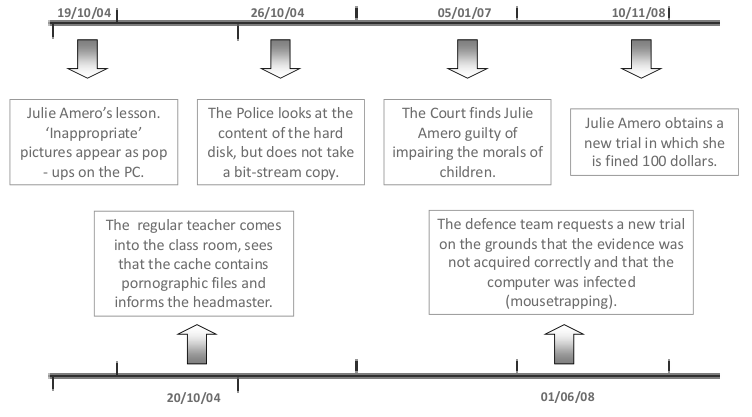
\includegraphics[width=1\textwidth]{img/amero_case.png}
    \caption{Timeline of the case}
    \label{fig:amero case}
 \end{figure}


\subsection{What is digital Forensics}

\textbf{Digital Forensics} is get hold of evidence without modifing the IT 
system in which that evidence is found, ensure that the 
evicence acuired in another medium is identical to the original and 
analyse data without modifyin it.

\subsection{The “Big Five” of Digital Forensics (Council of Europe)}

\begin{itemize}
    \item \textbf{Data Integrity:} No action taken \textit{should change electronic devices or media}, 
    which may subsequently be relied upon in court.
    \item \textbf{Chain of custody:} An \textit{audit trail} of all actions taken when handling electronic 
    evidence should be created and preserved
    \item \textbf{Specialist Support:} If investigations involving search and seizure of electronic 
    evidence it may be necessary to consult \textit{external specialists}. 
    \item \textbf{Appropriate Training:} First responders \textit{must be appropriately trained} to be able 
    to search for and seize electronic evidence if no experts are available at the scene
    \item \textbf{Legality:} The person and agency in charge of the case are responsible 
    for ensuring that \textit{the law and the above listed principles} are adhered to. 
\end{itemize}

\section{Digital Forensics Procedure}
Six phase of digital forensics procedure:

\subsection{Identify the Suspect}
There are 3 main phase for identify the suspect:

\begin{itemize}
    \item \textbf{Osint and Socmint:} Very usefull for collect information reguarding criminal 
    (even mafia ones), from social media, and other public sources.
    \item \textbf{Data Retension Directive in EU:} The investigator uses the Court 
    System to compel the ISP to reveal a physical location that 
    corresponds likely to the source of Network (IP Address)
    \item \textbf{Multiple User ID or multiple 
    Ips over time,  open Wi-Fi, Proxy, Botnet}: Under a warrant (depending from the Jurisdiction) 
    the location is searched and any computer or other device is seized
\end{itemize}

\subsubsection{Data Retension}
With the Directive 2006/24/EC, the EU member states are required to store data for 
a period of \textbf{6 to 24 months} (but can change from state to state). 
The data stored are gerally call detail records (CDR) of 
telephony and internet traffic and location data (IPDRs). \\
So evert single country and ISP have different data retention policy, and 
this can be a problem for the investigator, but from a privacy point of view a short time 
or null data retention is better.

\newpage

\paragraph{Transparency report:} Every year the ISP need to publish a transparency report 
where they show the number of request of data retention and the number of request that they 
have accepted.

\begin{figure}[h!]
    \centering
    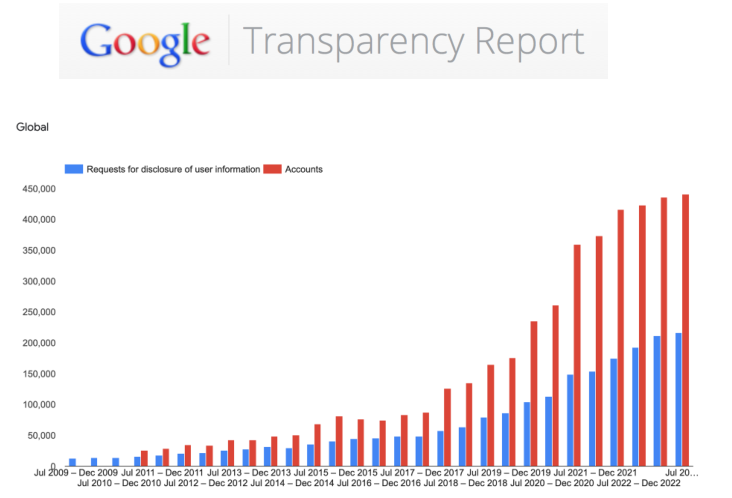
\includegraphics[width=0.6\textwidth]{img/transp_report.png}
    \caption{Timeline of Google transparency report}
    \label{fig:transparency report}
 \end{figure}

\subsubsection{Identify the suspect}
it's rigth use face recognision to identify a suspect? \\ 
For the moment if the situation is critical is possible utiliza A
live facial recognision. \\ 
AI act also regulate the use of facial recognision. % recuperare info dal testo del AI act

\subsection{Detecting and Seizing Digital Evidence}
The seize of digital evicences has torespet two foundamental rules: \textbf{bit-Stram Copy} and 
\textbf{Hash Function}. (definitions are alredy knowed)

\subsubsection{Where and how is the digital/electronic evidence hosted?}
The digital evicence can be in the suspected PC or in a third party server. \\
In the first case, we need to mange the encrition of the data, and it's possible get a Key Mandatory Law. \\
In the case of evicende in a server, is needed a collaborationfrom the ISP/Telco/Banck, and so need there is Jurisdiction problem. 

\subsubsection{The role of third paries during digital investigation}

A third party can give a lot of usefull information. \\
For example and \textbf{ISP} Could reveal from which place the email was sent, the \textbf{Mail Account Provider} could reveal from which places the email account was accessed and a \textbf{Credit Card Company} could reveal where the goods bought with a cloned credit card were delivered

\subsection{Validating Digital Evidence}
There is some tool that help to valdiate online digital evidence. \\
These kind of tool are usefull during OSINT bacasue they permit to collect data (like a story, a reel), that are not sure remain online, in a proper way for a court.


\subsection{Chain of Custody}

Digital storage media last less than analogue media and devices to read such media last even less. For example a LaserDisc last only 15 years, where there are books form thr 1086 (domesday book). So there at the moment, for trial, there are a lot of hard drive keeped in proprer way to avoid the data loss. It's a real mess.


\subsection{Analysis of Digital Evidence}

Start after the sieze of suspect's device, and need to be performed besided a precise chain of custody. \\ To perform the analysis are usually used some automatic tools, but in the recent time are used also some AI tools but only for post analysis and not for prediction policies (limitation imposed by the AI act) for example AI can not be used for kidnapping cases because the crime is in progress and not "finished".

\begin{itemize}
    \item \textbf{Text searches:} aimed at scanning files, directories and even entire file systems for specific text terms (generative AI can be used for summarizing and analyzing documents, but it's not very precise, plus alucination)
    
    \item \textbf{Image searches:} aimed at identifying image files in various formats, and at generating still frames of digitally stored video footage. Mainly analysis of child pornography that can be lead also to false positive (like a video of a mum and child in a bath)
    
    \item \textbf{Data recovery:} aimed at recovering all files stored on mass memory units, including deleted or damaged data. Destroy data can also be a crime (even if there are some backups), based on the intention of the crime (like delete file to hide evidence) 
    
    \item \textbf{Data discovery:} targeted at accessing hidden, encrypted or otherwise protected data
    
    \item \textbf{Data carving:} focused on reconstructing damaged files by retrieving portions of their content
    
    \item \textbf{Metadata recovery and identification:} this digital forensic tool is particularly useful for retracing the timeline of web accesses and file changes
\end{itemize}

Some other problem withthe use of \textbf{AI for prediction} of crime are: the bias of the AI and possible conseguences for privacy and \textbf{social control} by not very democratic government. 

\subsubsection{Two Italian issues}

\paragraph{Repeatable or Unrepeatable forensics analysis: }
\textbf{Repetable} when you can do a bit-stream copy of the data and also give one copy to the defence to do the same analysis, and more in general i can repeat analysis again and again (when i want). \\ In a \textbf{non-repetable} analysis, we need do live forensics activity and ofter occure with mobile phone, where there isn't the possibility to do a bit-stream copy of the data. In the live forensics i also need the presence of the attorney or the defender when i do the analysis to make it admissable in court.

\paragraph{Open Source or Closed Source:} %% recuperare da lezione
Open source can be more transparent 

\subsection{Presentation in Court}

The presentation of digital evidence findings is a \textbf{crucial stage} for prosecutors, judges, and lawyers (the evidence need to be presented in a way that the judge can understand it otherwire he can ignor it). The outcome of the trial relies not only on the results of the investigation but also on the \textbf{clarity and comprehensibility} of the report provided. \\

\textbf{Operational Recommendations:}
\begin{itemize}
    \item \textbf{Presence of an index:} The report should include a clear index for easy navigation through the document.
    \item \textbf{Glossary and Reference Notes:} If technical terms are used, a glossary and reference notes should be provided to ensure that all parties understand the terminology (judge and lawyers are not IT experts).
    \item \textbf{Timeline Table and Flow Charts:} A timeline table or flow charts should be included to visually represent the sequence of events and digital activities.
    \item \textbf{Presentation Slides with Photos:} Visual aids, such as presentation slides with photos, help in simplifying complex technical details.
    \item \textbf{Video Recording:} Where applicable, video recordings of the operations carried out during the investigation can provide further clarity.
\end{itemize}

\subsubsection{Presentation in Court of the Digital Evidence Findings: Murtha Case}

%% recuperare da lezione


\section{Privacy and Due Process Rights}

\subsection{Encryption}
Encryption can be used to hide the fact that encrypted messages are exchanged and used by criminals can lead to difficulties collecting the necessary evidence

\begin{figure}[!ht]
    \centering
    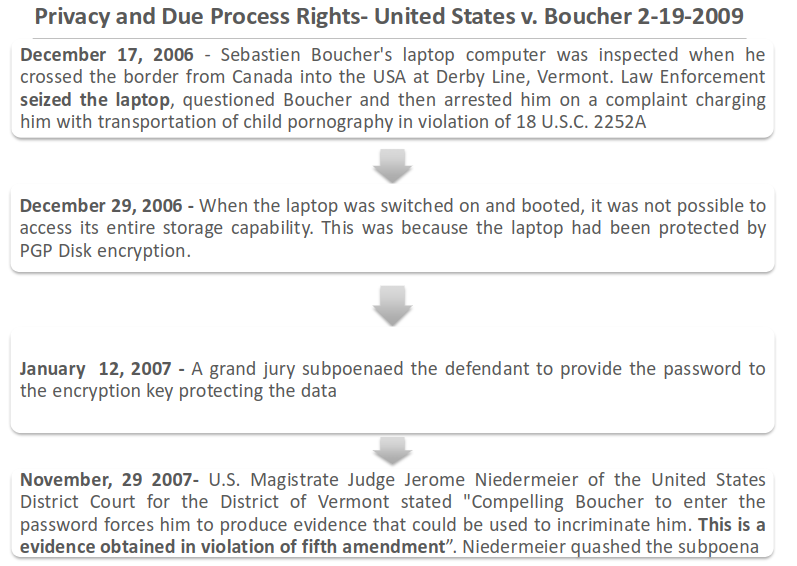
\includegraphics[width=0.5\textwidth]{img/enc_case.png}
    \caption{Case correlated with the use of encryption}
    \label{fig:encryption process}
\end{figure}

\newpage
\subsection{Case Law on Encryption}
Anther the previus case, some state are starting to create law about “Mandatory Key Disclosure" that force the suspect to give the key/password to decrypt the data. (some are Australia, Belgium France etc\dots) 

\subsection{Mandatory Key Disclosure Laws}
These case of legislative instrument doesn't work fow two main reason:
\begin{itemize}
    \item \textbf{technical reason:} An expert could always find a way yo hide a file
    \item \textbf{Possible violation of European Convention on Human Rights:} Article 6 Everyone charged with a criminal offence shall be presumed innocent until proved guilty according to law
\end{itemize} 

%% recuperare da lezione ---------

\subsection{Remote Forensics}

\begin{figure}[h!]
    \centering
    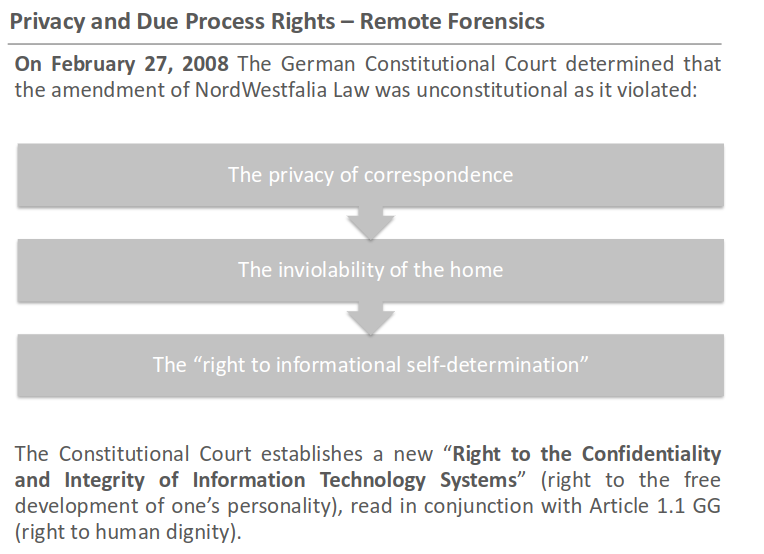
\includegraphics[width=0.4\textwidth]{img/remote_case.png}
    \caption{Case correlated to remote forensics}
    \label{fig:remote process}
\end{figure}

\subsection{Cloud Computing}

Cloud computing services face two key legal challenges: \textbf{Jurisdiction} and \textbf{Privacy}.

\paragraph{Jurisdiction}
The “\textbf{loss of location}” of digital evidence in the cloud introduces significant jurisdictional issues. In a cloud environment, the question arises: are the documents governed by the laws of the state in which they are physically located, the location of the company possessing them, or the laws of the state where the individual resides?

Over the last few years, various legal frameworks and approaches have been proposed to address this complex issue, but it remains an area of ongoing debate.

\paragraph{Privacy}
Cloud computing introduces several privacy concerns, including:
\begin{itemize}
    \item \textbf{Lack of Control:} Cloud clients may no longer maintain exclusive control over their data, limiting their ability to implement necessary technical and organizational measures to comply with \textbf{Data Protection Laws}.
    \item \textbf{Absence of Transparency:} Cloud providers may not provide sufficient information regarding how data is processed, leading to significant risks in terms of compliance with data protection regulations.
\end{itemize}


\subsubsection{Lack of control over the data} 
\begin{figure}[h!]
    \centering
    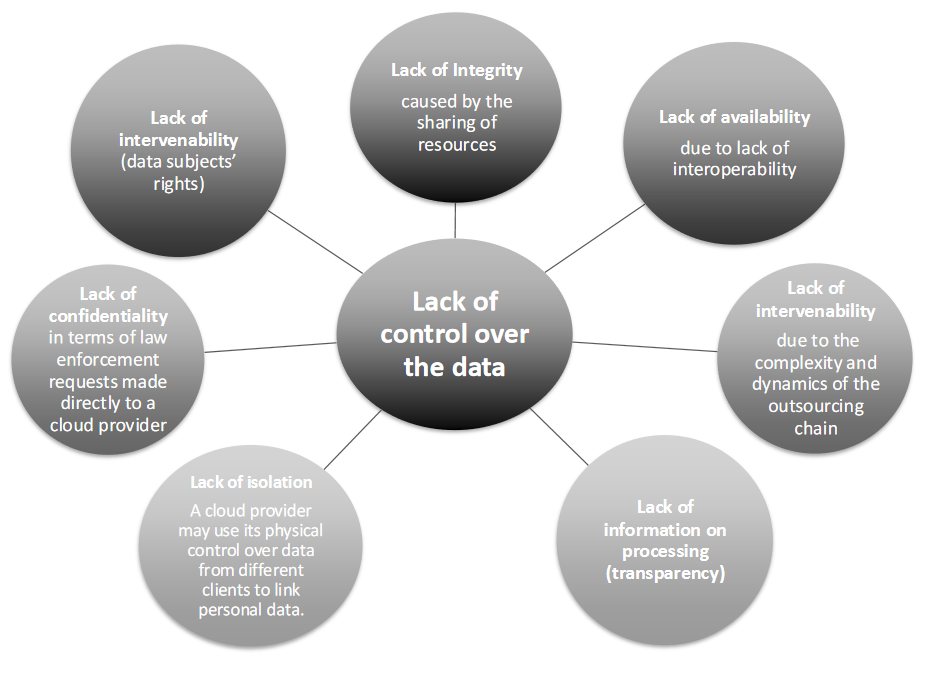
\includegraphics[width=0.5\textwidth]{img/cloud_lack_ctrl.png}
    \label{fig:lack_of_control}
\end{figure}



\subsubsection{Jurisdiction}  %% check, testo da GPT

In addressing the “loss of location” issue within the realm of cloud computing, we have four possible legal principles that can be applied:

\begin{itemize}
    \item \textbf{Territorial Principle:} The court in the jurisdiction where the data is physically located has authority. Jurisdiction is determined based on the geographical location of the data.
    
    \item \textbf{Nationality Principle:} The nationality of the perpetrator is used to establish criminal jurisdiction. The legal framework of the country of the individual committing the crime applies.
    
    \item \textbf{Flag Principle:} This principle applies to crimes committed on ships, aircraft, and spacecraft. They are subject to the jurisdiction of the country whose flag the vehicle flies under.
    
    \item \textbf{Power of Disposal Approach:} This approach focuses on who has control over the data. A regulation based on this would enable law enforcement to access a suspect's data in the cloud, regardless of its physical location, by considering the individual or entity with power over the data.
\end{itemize}

%% ------------------------------------
\chapter{Convention on Cybercrime}

\section{E-commerce on Dark Web}

\subsection{Silk Road}

\section{History and objectives of the Convention on Cybercrime (Budapest Convention)}

\subsection{Budapest Convention on Cybercrime }
%% overview direttamente nella section

\subsubsection{Timeline and Ratifications}

\subsubsection{Criticism and Opposition}


\subsection{New Global Cybercrime Treaty (UN, August 8, 2024)}

\subsubsection{Aim of the convention}

\section{Harmonization of national laws and international cooperation}



\part{Tech}
\chapter{Introduction}

\section{Topics}
\begin{itemize}
  \item \textbf{Forensics Analysis} \\
    use of logic and meaningful knowledge and methodological approach to
    legal problems and criminal investigation.
  \item \textbf{Computer Forensics} \\
    Collection, preservation and analysis of digital evidence
    (inside file system, email, cloud account etc...) to support
    investigation and legal proceedings
\end{itemize}

\section{Forensics History}

\subsection{Ancient Times}
Forensic science dates back to \textbf{Babylon (1900 BC)} where fingerprints
were used for identification, and \textbf{China (1248 AC)} with forensic pathology.
In the \textbf{UK (1835)}, bullet comparison solved a case, and by \textbf{1892},
the first murder was solved using fingerprints.

\subsection{Modern Times}
Forensic standards grew in police departments, with the first crime lab in
\textbf{1923}. DNA fingerprinting began in the \textbf{1950s}, and DNA profiling
was developed by \textbf{1985}. \textbf{AFIS} systems emerged in the late
\textbf{1980s}. Today, AI, toxicology, and digital forensics are key areas
of innovation.

\subsection{Digital Field}

\subsubsection{Early Times}
In \textbf{1989}, Robert Morris was convicted under the Computer Fraud and
Abuse Act, marking the first use of computer logs in forensics. That year,
\textbf{IACIS} was founded, followed by \textbf{IOCE} in \textbf{1995} to
share digital forensic practices.

\subsubsection{Recent Times}
\begin{itemize}
  \item \textbf{1990}: Forensic tools like EnCase emerged
  \item \textbf{2000}: Digital forensics became widespread in law enforcement
  \item \textbf{2010}: Growth of cloud and mobile forensics, automation, and
    machine learning
  \item \textbf{2020}: Advances in crypto, blockchain, and AI improve digital
    forensics
\end{itemize}

\section{Computer Forensics Definitions}

\textbf{US\_CERT:} The discipline that combines elements of law and computer
science to collect and analyze data from computer systems,
networks, wireless communications, and storage devices in a
way that is admissible as evidence in a court of law. \\
\textbf{A. Ghirardini -Computer Forensics:} The discipline whose goal is preservation, identification, analysis of
information system to the aim of identification of evidences during
investigation activities. \\
\textbf{NIST glossary:} The application of computer science and investigative procedures
involving the examination of digital evidence - following proper search
authority, chain of custody, validation with mathematics, use of validated
tools, repeatability, reporting, and possibly expert testimony.

\section{CF purpose(s)}

\subsection{CF Q\&A}
During an investigation, digital forensics need to analysis data to answer some key questions: \\
\begin{minipage}[t]{0.45\textwidth}
  \begin{itemize}
    \item \textbf{What happened?}
    \item \textbf{Who was involved?}
    \item \textbf{When did it take place?}
  \end{itemize}
\end{minipage}
\begin{minipage}[t]{0.45\textwidth}
  \begin{itemize}
    \item \textbf{Where did it take place?}
    \item \textbf{Why did it take place?}
    \item \textbf{How did an incident occur?} \newline
  \end{itemize}
\end{minipage}

The answers to these questions are essential for support legal proceedings and mitigate
possibility of future incidents with a preventive approach.

\subsection{CF Goals}

The goals of computer forensics (CF) are multifaceted and aim to provide a
comprehensive understanding of digital incidents. \\
Firstly, CF seeks to retrieve what has been the input, such as what has been typed.
It also aims to determine the actions performed, for example, what programs have been run
and what peripherals have been connected. \\
Additionally, CF involves analyzing used files to understand what modifications
have been done and when these modifications occurred (and the information from an OS
  are not enougth, because are an abstraction managed by the file system $\rightarrow$ needed
bit analysis (like for ereased data)). \\
Another critical goal is to identify the damage done,
such as what data have been erased. In essence, the overarching goal
of CF is to \textbf{gain a technical comprehension of what happened during the
incident} (from a technical point of view).

\chapter{CF Terminology \& revelant conceps}

\section{Terms}

\subsection{Digital evidence}
Technical definition of Digital evidence is very similar to the legal ones:
\begin{boxH}
  Data stored or transmitted in digital form that can be used in court.
\end{boxH}

The conrnerstones of digital forensics are the different levels of \textbf{abstraction}, requires
\textbf{interpretation}, are \textbf{fragile}, may be \textbf{voluminous}
and the difficulty to discover \textbf{connection} between
data and reality (the connection need to be done beafore entering the court). \\

Digital evidence also requires a deep technical understanding of the possible types of data
(files, emails, logs, metadata) and the legal requiremnets for each of one to collect and preserve it.
(To make all of this effective, knowledge of file systems, network protocols
and encryption are essential) \\

\subsection{Chain of custody}
\begin{boxH}
  Documented and \textbf{unbroken} process of handling evidence
  from the time it is collected until it is presented in court
\end{boxH}

This procedure is essential to ensure the integrity of the evidence and to avoid
that them to be tampered or accessed by unauthorized people. \\
Keep the chain of custody requires knowledge about how to document evidence
collection, storage, and access (logging procedures, secure storage, legal prtocols etc..) \\

If the chain of custody is \textbf{broken}, the evidence may be considered \textbf{inadmissible in court}
(so is needed know the regulation of the state to decide how to manage it).

\subsection{Data acuisition}
\begin{boxH}
  The process of collecting digital evidence from devices
  without altering or damaging the original data.
\end{boxH}

One of the biggest problem fo the managment of digital evidence, because it's needed to be performed
on hostile systems (that can be infected, compromised, have a malware or system to avoid copy
like edited system call for make other program to fail). in a not coltrolled envorment like a crime scene. \\
So are needed knowledge of disk imaging and live data capture in order to not alter what's going on
on the suspect system. Are also required expertise in forensics acquisition, analysis
tools (like FTK Imager, EnCase) and knowledge of file systems, write-blockers, and hashing
(crucial for ensuring integrity).

\subsection{Hashing}
\begin{boxH}
  The process of converting data into a fixed-length string of
  bits, which represents the data uniquely
\end{boxH}

It's used in the chain of custody for ensure the integrity of the digital evidence and so verity
that a file has not been altered. \\
Require understanding of hashing algorithms (strengths and
weaknesses, e.g. MD5 collision), formats
(hex, base64 etc...) (if wrong formats are sued, the chain of custody is broken and each information
gathered from that point is considered not valid)
and expertise in hashing tools (sha256sum, hashdeep, FTK imager, Autopsy). \\

Have to be used any time an evidence is "managed" (copied, moved)

\subsection{Write Blocker}
\begin{boxH}
  Hardware or software tool used to prevent any data from
  being written to a storage device during analysis, preserving
  the original data content
\end{boxH}

To be operated, require understanding of how write-blocking devices work
and how they can be implemented in forensic procedures. \\

It's essential for the legally defensible acquisition.

\subsection{Forensic image}

\begin{boxH}
  A bit-by-bit copy of digital media, including deleted files and
  data in slack space, which is an exact replica of the original device
\end{boxH}

The goal of a forensic image is to preserve the original evidence and aovid the modification
of the original data. \\

To be performed in a correct way, requires understanding of mechanisms to copy information
in digital devices (file system knowledge and behavior) and familiarity with  with bit-by-bit copy tools
(DD, FTK Imager, EnCase, Guymager). \\

As the hashing, it's need to be used any time an evicene is "managed" (copied, moved)

\section{Scenarios}
There are some possible scenario that a computer forensic investigator can face:
\begin{itemize}[itemsep=0pt]
  \item Internet abuse from employee
  \item computer-aided frauds
  \item Data unauthorized manupulation (theft or destruction)
  \item Computer/network manage assessment
  \item \dots any other case that include digital evidence
\end{itemize}

\section{investigation phases}

A Computer forensics investigatos usually follow standard phases that guide him. There are different standards like: NIST family, ACPO guidelines (UK), ISO/IEC 27042, SWDGE.

\subsection{Phases}

\begin{itemize}[itemsep=0pt]
  \item \textbf{identification:} When the investigator come for the first time to the crime scene and need to identify potential source of relevant digital evicences.

  \item \textbf{collection:} The letteral pick up of the evidence (like a computer or a smartphone) or a remote taking possession of the evidence (like for a remote server) and its connection (e.g. network or physical, like USB disk). \\ It's splitted from acquisition because it's a critical phase where the evidence can be altered and lost utility for the investigation (es. data corruption, lost of metadata etc...)

  \item \textbf{acquisition:} Electronically retrieving data by running various CF tools and software suites

  \item \textbf{evaluation:} Evaluating the data recovered to determine if and how it could be used against the suspect (e.g. for prosecution in court)

  \item \textbf{presentation:} Presenting the evidence discovered in a manner which is suitable for lawyers, non-technical staff/management and the law (and internal rules)
\end{itemize}

\subsection{Identification}
During the identification phase is important \textbf{recognize} all the \textbf{relevant data sources} before any acquisition, even if no physical present, like data in the cloud \\ A imple \textbf{list of example} are: hard drives (HDD/SSD), memory (RAM), mobile devices (smartphones, tablets), cloud storage, network traffic, removable media (USB drives, DVDs), IoT devices and embedded systems (like smart washing machines) \\
\bigskip For identify these sourcer, the investigator can perform some actions, like:
\begin{itemize}[itemsep=0pt]

  \item Perform an initial survey of the scene (physical or network environment)

  \item Identify key devices and data locations (local storage, remote servers, cloud services)

  \item Check for connected devices, including peripherals like printers, removable media, or network-attached devices

  \item Map all potential data sources using network topology diagrams or asset inventories

\end{itemize}

A particolar aspect that need to be considered is the possible present of "ephemeral" storage or data, like cloud syncing, hidden secttor, tmp, dat in ram etc...

\subsection{Collection}
During the collection, the focus is on gathering evidence from identified data sources while ensuring the preservation of its integrity. An important key point is the implementation of methods that \textbf{minimize the risk of evidence tampering or data loss}. \\
For enforce this key point, it's importnat \textbf{isolate devices} to prevent them from being tampered with remotely (e.g., disconnect them from the network), use devices to \textbf{block external
communication} for mobile or wireless devices and use network isolation tools for virtual and cloud environments to prevent remote access (like use a virtual private cloud). \\
A particular note is for the managment of live systems where is needed ensure evidence integrity while
maintaining system uptime (so not shoutting down the system for avoid the loss of volatile data). \\
Create a \textbf{detailed record} of the condition and state of the evidence
\begin{itemize}[itemsep=0pt]
  \item take photographs of the devices in situ, including connected peripherals and the physical state
  \item  record serial numbers, device models, and any other identifiable information
  \item  document the scene, noting which devices were running, whether screens were active o locked, and any other visible indicators
\end{itemize}
\textbf{hint:} complete documentation is crucial to prevent legal challenges regarding the integrity of the evidence. \\
Beafore procede to the acquisition, is needed to ensuring no alteration will take place, so do somethings like enable write blockers for physical storage devices, disalbe connection and sinking. particulary complex is maintain  integrity on live systems (e.g., using remote collection methods that minimize data alteration risks)

\subsection{Acquisition}
The act of performing a forensic copy (so a bit-by-bit copy) of the original data with the goal of ensure that the acquired data is a faithful replica of the source so to maintaining data integrity. \\
There 2 two main acquisition methods:
\begin{itemize}
  \item \textbf{Static:} When the system is powered down, it's se most commod method for acquiring data from hard drives and extenral memory
  \item \textbf{Live:} The system is running and it's needed to deal with volatile data like RAM, network connections, or running processes.
\end{itemize}

\subsubsection{Static acquisition}
\begin{enumerate}
  \item shut them down carefully to avoid losing data \\
    • e.g. for encrypted devices, consider methods for capturing data without triggering loss of access (e.g., before the decryption key is wiped from RAM)
  \item attach the device to a forensic workstation using a write blocker
  \item use forensic imaging tools to create a complete image of the storage device
  \item generate a hash value (e.g., SHA-256) of the original media before and after acquisition to verify integrity
  \item store the image on a secure forensic storage device
\end{enumerate}
\textbf{hint:} pay attention that data is properly hashed and verified post-acquisition, not perform steps like an automata.

\subsubsection{Live acquisition}
\begin{enumerate}
  \item choose a method that minimizes system interference while capturing volatile data
  \item dump RAM (memory acquisition) and capture data from running processes or network connections.
  \item perform network traffic capture
  \item document all acquisition actions and steps to ensure chain of custody and admissibility
  \item hash the volatile data wherever possible to maintain data integrity
\end{enumerate}

\subsubsection{Integrity}
In this phase is needed to ensure that the acquired data is an exact replica of the original and has not been altered. \\ Performed mainly by the use of hashing algorithms. \\ Some general steps are:
\begin{itemize}[itemsep=0pt]
  \item choose a method that minimizes system interference while generating a hash (MD5, SHA-256) of the acquired image or data dump
  \item compare the hash value to the original data hash (for static data) to verify its integrity
  \item document the hashing process, including the algorithms used and the results, in the chain of custody documentation
\end{itemize}
\textbf{hint:} be careful! any discrepancies in hash values would require re-acquisition and could damage the credibility of the evidence

\subsubsection{Chain of custody}
This section need to be performed in paralled with all the other phases to ensure a complete, documented chain of custody for the evidence throughout the acquisition process. (Record every step in the acquisition process, including personnel involved, tools used, date, and time of acquisition. \\ Store the data and evidence securely to avoid unauthorized access or tampering)

\subsection{Evaluation}
analyzing, verifying, and validating the evidence to ensure it remains unaltered and trustworthy for legal proceedings or further analysis. It's possible alter the evidence only if the evaluation is performed on a copy of the original data. \\
More in practice, the main actions that are performed are:
\begin{itemize}[itemsep=0pt]
  \item timestamp and metadata analysis
    \begin{itemize}
      \item verify file creation, access, and modification dates of data to ensure they match the timeline of the incident
    \end{itemize}
  \item timeline reconstruction
  \item cross-reference analysis/consistency verification
    \begin{itemize}
      \item correlation of digital evidences with external logs or other data to countercheck it is related to the suspected system or device
      \item comparison of data from different sources (e.g. logs, email)
    \end{itemize}
  \item compliancy with current legal/internal standards
    \begin{itemize}
      \item collection, preservation, evaluation must be coherent to applicable legal procedures...and the documentation must keep track of that
    \end{itemize}
  \item review of possible anti-forensics techniques
\end{itemize}

\subsection{Presentation}
Preparing and presenting the findings of the investigation in a clear, accurate, and legally admissible manner is essential. The goal is to \textbf{translate} the technical details of the forensic analysis into a format that can be understood by \textbf{non-technical stakeholders}, such as lawyers, judges, or company executives.

\textbf{Hint:} The quality and clarity of the presentation can significantly influence the outcome of legal proceedings or internal investigations.

\subsection*{Actions:}
\begin{itemize}[itemsep=0pt]
  \item Review all the data collected, analyzed, and interpreted during the investigation.
  \item Identify the key pieces of evidence.
  \item Verify that all conclusions are directly correlated to verifiable evidence.
  \item Document the entire forensic process in a formal report, free from technical jargon, so that it can be submitted as legal evidence.
  \item Securely manage the report to ensure its integrity.
\end{itemize}

\subsection*{Hints:}
\begin{itemize}[itemsep=0pt]
  \item Avoid "personal interpretation" unless explicitly asked to provide expert opinion.
  \item Include appendices with timestamps, metadata, hash values, and other forms of technical evidence as "reinforcement."
\end{itemize}

\chapter{Non-trusted environment issues}
We need to not trust an enviroment by default, becasue it can be compronised, and there are many ways to do so.

\section{Compromise causes}
\subsection{Node infection}
Nowadays, a node infection is obtained through a social engineering attack, that lead to the download of a compromise file/software.
\begin{itemize}[itemsep=0pt]
  \item Legitimate software containing malicious code (trojan horses) (a free version of paied software is alsways a good bait), social engineering, physical access, bug or configuration error exploitation (OS syscall, device driver, application, firmware and BIOS, browser ...)
  \item Backdoors creation, data stealing, hidden (or not so much) processes disruption, …
  \item Persistent unauthorized access to a system (as root - i.e. rootkits)
  \item Spyware (sensitive information collection)
  \item Ransomware (encryption of sensitive data)
\end{itemize}

\subsection{network injection}
\begin{itemize}[itemsep=0pt, topsep=0pt]
  \item nodes capable to read and write data while in transit, actors capable to "poison" routing mechanisms
  \item access and modification of network data flow, redirection versus illegitimate destination
  \item Sniffers and (growing) family of Man-in the-X  attacks$_{\ref{sec:Mitx}}$
\end{itemize}

\subsection{supply chain attacks}
\begin{itemize}[itemsep=0pt, topsep=0pt]
  \item compromise of service, hardware, software of a third-party vendor or partner used (and trusted) by the target organization
  \item gain access to the target organization, inject unauthorized behavior
  \item infrastructure for update management
  \item
    \begin{itemize}[itemsep=0pt, topsep=0pt]
      \item e.g. SolarWind Orion Attack
      \item malicious code into software updates of Orion network monitoring platform.
      \item distributed to over 18,000 customers, including government agencies and large corporations.
    \end{itemize}
  \item libraries and dependencies
  \item hardware during manufacturing
  \item IT infrastructure management service
  \item ...
\end{itemize}
\subsection{Men at work} \label{sec:Mitx}

\subsubsection{man-in-the-middle}
An attacker secretly intercepts or alters communication between two unaware parties. \\Examples include \textbf{HTTP session hijacking}, where the attacker intercepts session cookies to impersonate a user, and \textbf{ARP table poisoning}, where ARP tables are altered for traffic redirection.

\subsubsection{man-in-the-browser}
Infection occurs in the browser to alter web pages or transactions.\\ An example is banking trojans like \textbf{ZEUS}, which modify online transactions.

\subsubsection{man-in-the-cloud}
This involves stealing credentials or tokens to access a user's cloud environment.\\ For example, the interception of a Google Drive OAuth token can allow access to the victim's files.

\subsubsection{man-in-the-mobile (MitMo)}
Mobile infection is used to intercept communication or two-factor authentication (2FA).\\ An example is ZitMo, which intercepts SMS and forwards them to a command and control (C\&C) server.

\subsubsection{man-in-the-disk}
This exploits vulnerabilities in handling external storage.\\ For instance, an attacker can modify temporary files stored on an external device.

\subsubsection{man-in-the-memory (MitMem - guest star)}
In this case, an attacker intercepts or modifies data while it is in RAM.\\ A notable example is fileless (stealth) malware.

\subsubsection{man-on-the-side}
An attacker observes and injects communication without modifying it.\\ An example is China's Great Cannon.

\subsubsection{man-at-the-end}
This type of attack compromises end-point communication.\\ For example, a keylogger infection can capture sensitive information.


\section{Advanced persistent threats (APT)}
\begin{itemize}[itemsep=0pt, topsep=0pt]
    \item \textbf{advanced}
    \begin{itemize}[itemsep=0pt, topsep=0pt]
        \item use of sophisticated techniques
        \begin{itemize}[itemsep=0pt, topsep=0pt]
            \item customised malware, zero day vulnerabilities, evasion stategies
        \end{itemize}
        \item targeted to specific victim
        \begin{itemize}[itemsep=0pt, topsep=0pt]
            \item high budget and expertise, careful preparation
        \end{itemize}
    \end{itemize}
    \item \textbf{persistent}
    \begin{itemize}[itemsep=0pt, topsep=0pt]
        \item Item compromise maintained for extended period
        \begin{itemize}[itemsep=0pt, topsep=0pt]
            \item possible escalation and infection diffusion
        \end{itemize}
        \item low-profile operation (during infection)
        \begin{itemize}[itemsep=0pt, topsep=0pt]
            \item stealth techniques, limited bandwidth usage, mimicking legitimate traffic
        \end{itemize}
    \end{itemize}
    \item \textbf{threat}
    \begin{itemize}[itemsep=0pt, topsep=0pt]
        \item highly skilled individual aiming strategic goals (espionage, foreign country intelligence, …)
    \end{itemize}
\end{itemize}


\subsection{APT Attack Process}

The Advanced Persistent Threat (APT) attack process consists of several key stages:

\subsubsection{Initial Intrusion}
The attacker gains access through a weak entry point, such as exploiting zero-day vulnerabilities or using spear phishing techniques to infiltrate the target system.

\subsubsection{Foothold Establishment}
Once access is gained, the attacker sets up persistent access by installing backdoors or infecting the system with (stealth) malware to maintain control over the compromised environment.

\subsubsection{Privilege Escalation}
The attacker escalates privileges to gain further control over the target system. This involves techniques like credential stealing or vulnerability exploitation.

\subsubsection{Lateral Movement}
The infection spreads across the target organization as the attacker moves laterally, using stolen credentials or exploiting vulnerabilities to compromise additional systems.

\subsubsection{Goal Achievement}
The attacker eventually reaches their goal, which often involves data exfiltration or sabotaging critical systems.


\subsection{APTxx}

\textbf{APTxx} refers to organized hacker groups involved in advanced persistent threat (APT) activities. An example of such a group is \textbf{APT28}, also known as Fancy Bear.

\subsubsection{APT28 (Fancy Bear)}
APT28 is a Russian state-sponsored group that operates during Russian business hours and closely aligns with Russian government strategic interests, particularly in regions like the Caucasus. The group has been active since the mid-2000s, with documented operations dating back to at least 2008. APT28 targets a wide range of sectors, including aerospace, defense, energy, government, media, and dissidents, engaging in activities such as espionage, political influence, and cyberwarfare.

\paragraph{Notable Attacks:} In 2016, APT28 was responsible for the breach of the \textbf{Democratic National Committee} (DNC) during the U.S. presidential election. This attack led to the leakage of sensitive information with the intent of influencing the election outcome. \\Another major attack occurred in 2017 with the NotPetya ransomware, which was initially designed to target \textbf{Ukrainian institutions}. However, the malware spread globally, causing billions of dollars in damages.


\subsubsection{APT28 Typical Behavior}

APT28 targets a wide range of devices, including desktops, laptops, and mobile phones. It often employs \textit{(spear-)phishing} messages to direct victims to realistic websites for credential harvesting. 

\begin{itemize}
    \item APT28 registers domains that closely resemble legitimate organizations (e.g., \texttt{qov.hu.com} for the Hungarian government \texttt{gov.hu}).
    \item It uses URL-shortening services to obscure the true destination of malicious links.
\end{itemize}

In addition, APT28 delivers highly-realistic and targeted emails, often containing "weaponized" attachments such as \texttt{.docx} or \texttt{.pdf} files. These emails are designed to implant custom malware, such as \textbf{X-Agent}, a multi-functional malware implant used for:
\begin{itemize}
    \item Data exfiltration,
    \item Keystroke logging, and
    \item Multiplatform operations (Windows, Linux, Android, and iOS).
\end{itemize}

After gaining initial access, APT28 actively seeks to harvest credentials through techniques like keylogging and central memory dumping. To evade detection, APT28 adopts various evasion techniques, including:
\begin{itemize}
    \item Malware code obfuscation,
    \item Use of compromised certificate signatures,
    \item \textit{Timestomping} (modifying timestamps), and
    \item Encrypted communication channels.
\end{itemize}

APT28 also engages in \textbf{lateral movement} within the compromised organization by exploiting harvested credentials. This lateral movement involves:
\begin{itemize}
    \item Remote Desktop Protocols (RDP),
    \item Windows Management Instrumentation Command-line (WMIC) and \texttt{PsExec} to execute commands on remote Windows machines, and
    \item \texttt{SSH} to connect to remote Linux systems.
\end{itemize}

Finally, APT28 escalates privileges by exploiting harvested credentials or vulnerabilities in the system. \\

APT28 frequently engages in \textbf{data exfiltration} using custom \textbf{Command-and-Control (C2)} communication frameworks, such as \textbf{Zebra C2}. The exfiltrated data may be optionally compressed, especially if large, and is transmitted via encrypted channels like \texttt{HTTPS}, \texttt{FTPS}, or even custom protocols.

Although primarily known for espionage, APT28 has also been involved in \textbf{destructive attacks}. These include the use of \textbf{wiper actions}, such as:
\begin{itemize}
    \item \textbf{KillDisk}, designed to destroy the master boot record, and
    \item Disk wiping tools, particularly in the energy sector.
\end{itemize}


\section{Trusted Environment}

\subsection{(example of) System Call Interception}

\subsection{Examples of Linux system modification}


\end{document}

% Sample of a centered image in LaTeX
% \begin{figure}[h]
%     \centering
%     \includegraphics[width=0.5\textwidth]{path/to/image.png}
%     \caption{Sample Image}
%     \label{fig:sample_image}
% \end{figure}
